% !TeX root = main.tex
\documentclass[11pt,a4paper,UTF8]{ctexart}
\usepackage{quicklatex} % 引入自定义样式

\title{Quick \LaTeX 模板}
\author{张晋 \\ \url{theigrams@buaa.edu.cn}}
\date{\today}

\begin{document}



\maketitle
\tableofcontents
\newpage

\section{基础用法}

\subsection{表格}
表~\ref{tab:abl-traj} 来自~\cite{hu2023uniad}.

\begin{table}[htp]
	\begin{center}
	    \centering
        \scalebox{1}{
			\begin{tabular}{l|cccc|cccc}
				\toprule
				ID & \begin{tabular}[c]{@{}c@{}}Scene-l.\\ Anch.\end{tabular} &  \begin{tabular}[c]{@{}c@{}}Goal\\ Inter.\end{tabular} & Ego $Q$ &  NLO. &  minADE$\downarrow$ & minFDE$\downarrow$ & MR$\downarrow$ & \begin{tabular}[c]{@{}c@{}}minFDE\\ -mAP$^\ast$\end{tabular}$\uparrow$  \\
				\midrule
				1 &  &  &  & & 0.844 & 1.336& 0.177& 0.246\\
				2 & \cmark  & &  &  & 0.768 & 1.159& 0.164 & 0.267\\
				3 & \cmark  & \cmark&  &  & 0.755& 1.130& 0.168 & 0.264\\
				4 & \cmark  & \cmark &\cmark & & 0.747 &1.096 & 0.156& 0.266\\
				5 & \cmark  & \cmark & \cmark & \cmark& \textbf{0.710} &\textbf{1.004} & \textbf{0.146} & \textbf{0.273}\\
				\bottomrule
			\end{tabular}
		}
	\end{center}
	\vspace{-15pt}
	\caption{\textbf{Ablation for designs in the motion forecasting module.} All components contribute to the ultimate performance. ``Scene-l.\,Anch.'' denotes rotated scene-level anchors. ``Goal Inter.'' means the agent-goal point interaction. ``Ego $Q$'' represents the ego-vehicle query and ``NLO.'' is the non-linear optimization strategy. $\ast$: A metric considering detection and forecasting accuracy simultaneously, and we put details in the Supplementary.}
	\label{tab:abl-traj}
\end{table} 

\subsection{图片}
图~\ref{fig:pano_quali_supl} 来自~\cite{carion2020end}. 更多参看 \href{https://www.overleaf.com/learn/latex/How_to_Write_a_Thesis_in_LaTeX_(Part_3)%3A_Figures%2C_Subfigures_and_Tables#Subfigures}{How to Write a Thesis in LaTeX (Part 3): Figures, Subfigures and Tables}.
\begin{figure}[htp]
    \centering
     \begin{subfigure}[t]{\textwidth}
       \centering
       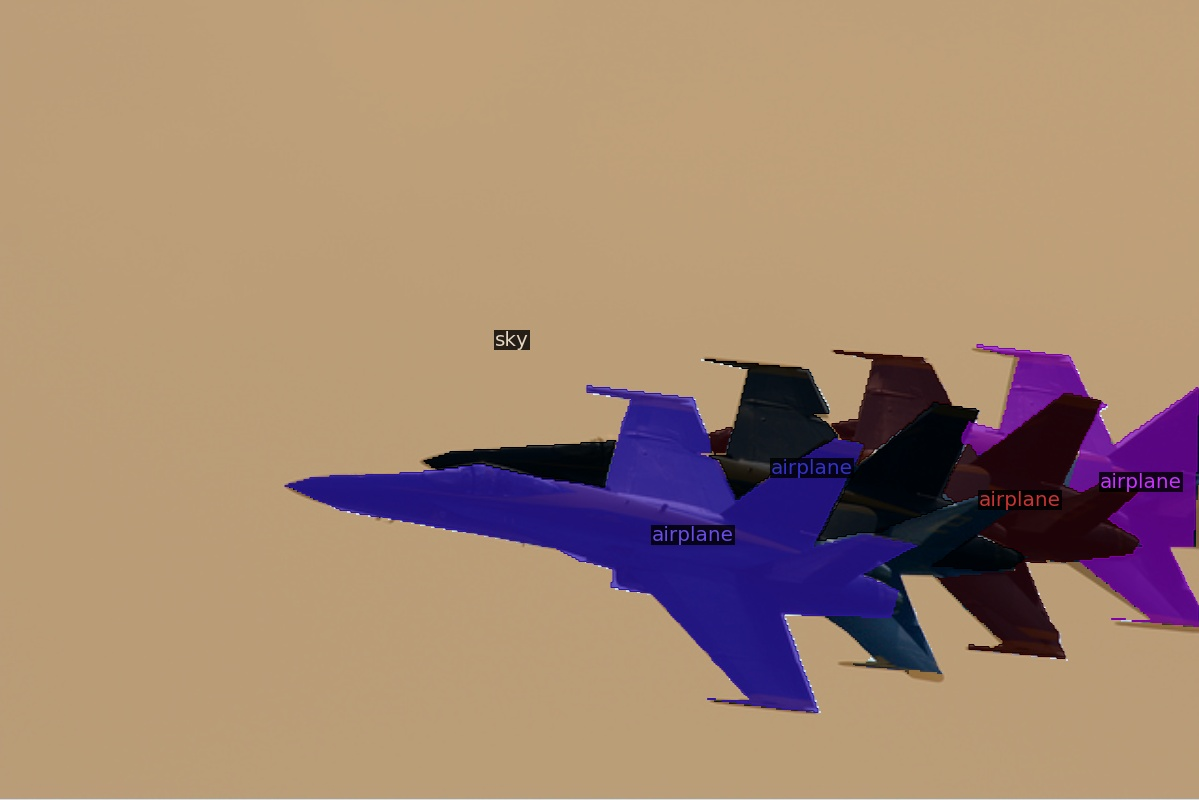
\includegraphics[width=.32\textwidth]{img/Panoptic/1113_gt.jpg}
       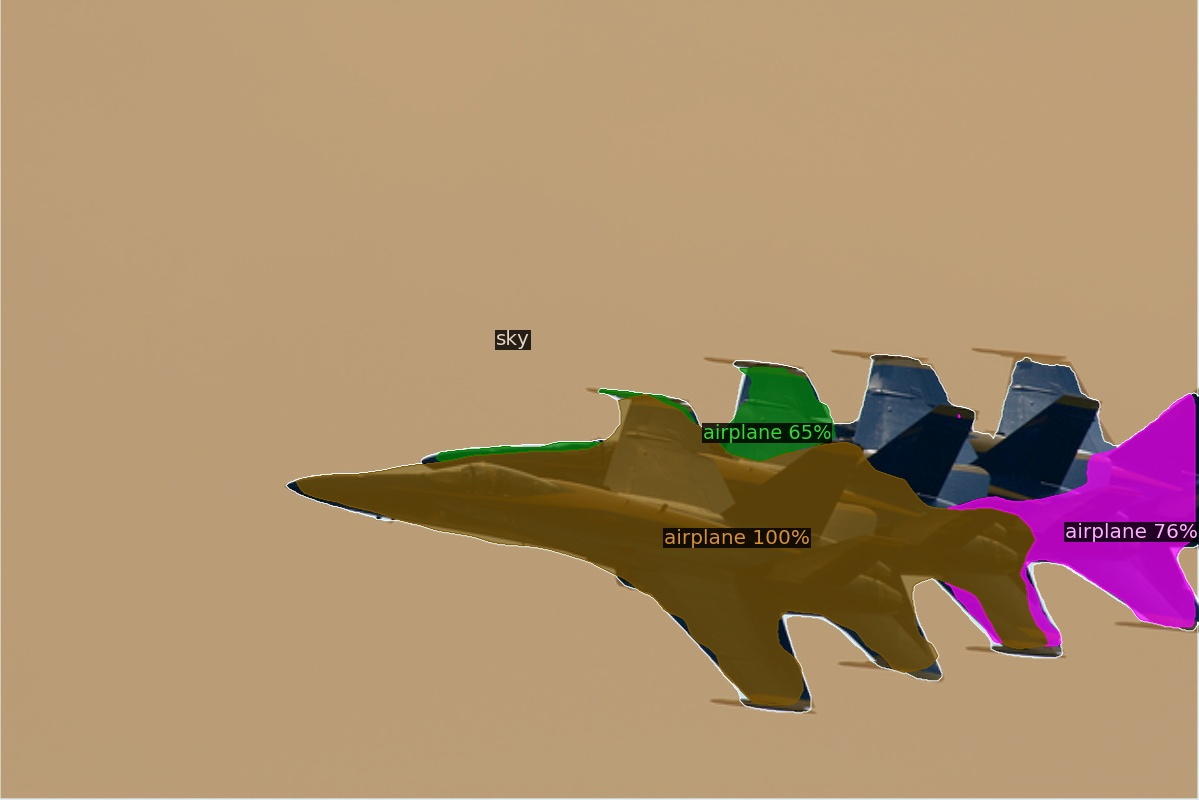
\includegraphics[width=.32\textwidth]{img/Panoptic/1113_panopticfpn.jpg}
       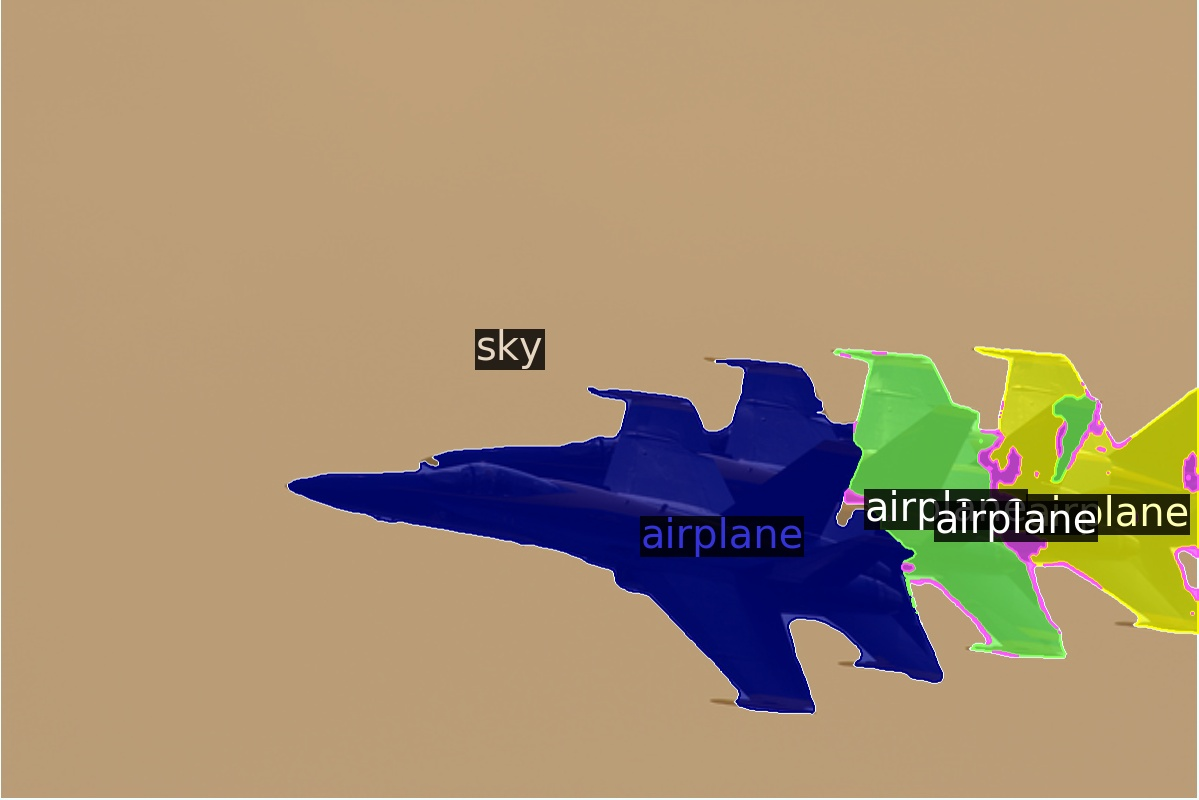
\includegraphics[width=.32\textwidth]{img/Panoptic/1113_detr_R101.jpg}
       
       
       \caption{Failure case with overlapping objects. PanopticFPN misses one
         plane entirely, while DETR fails to accurately segment 3 of them.}
     \end{subfigure}
    \ \\
    \begin{subfigure}[t]{\textwidth}
        \centering
        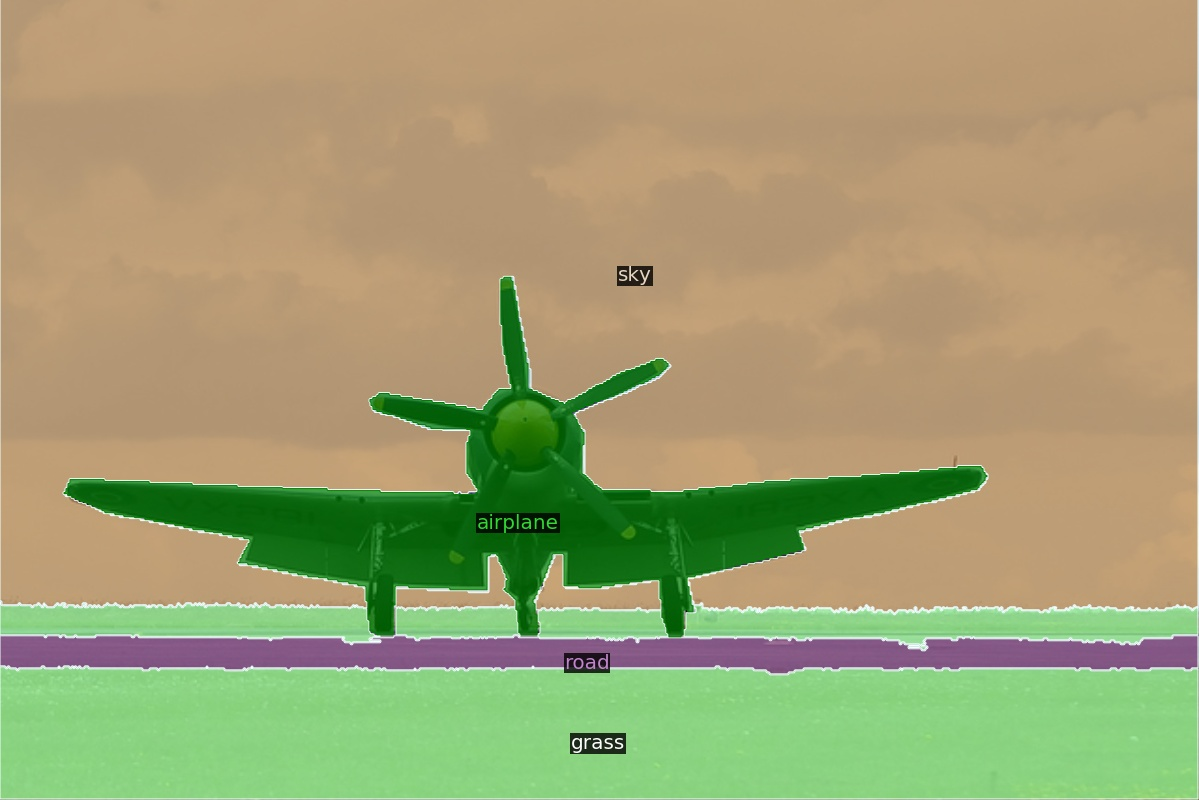
\includegraphics[width=.32\textwidth]{img/Panoptic/3485_gt.jpg}
        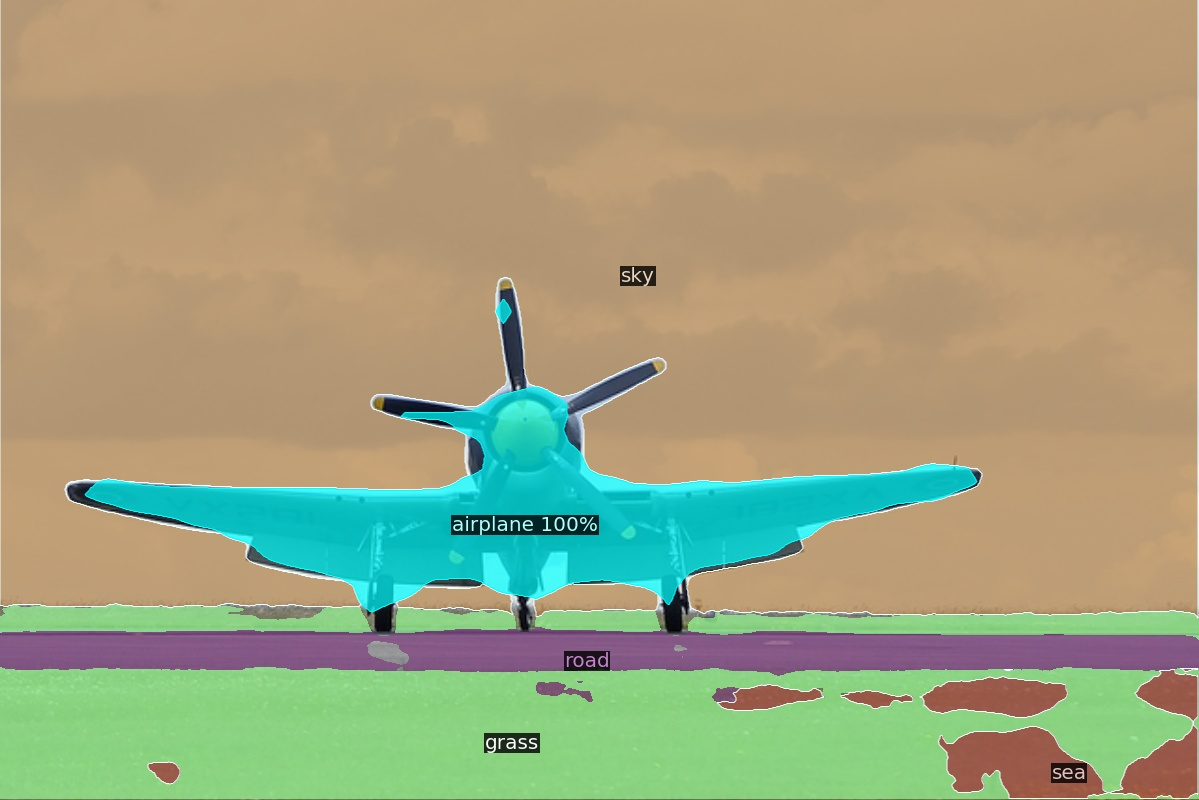
\includegraphics[width=.32\textwidth]{img/Panoptic/3485_panopticfpn.jpg}
        
\includegraphics[width=.32\textwidth]{img/Panoptic/3485_detr_R101.jpg}
        
        
        \caption{\texttt{Things} masks are predicted at full resolution, which allows sharper boundaries than PanopticFPN}
    \end{subfigure}%
\caption{Comparison of panoptic predictions. From left to right: Ground truth, PanopticFPN with ResNet 101, DETR with ResNet 101}
\label{fig:pano_quali_supl}
\end{figure}

\newpage
\subsection{数学公式}

\subsubsection*{矩阵}
\begin{lstlisting}[style=latex]
\begin{bmatrix}
    a_{11} & a_{12} & \cdots & a_{1n} \\
    a_{21} & a_{22} & \cdots & a_{2n} \\
    \vdots & \vdots & \ddots & \vdots \\
    a_{m1} & a_{m2} & \cdots & a_{mn} \\
\end{bmatrix}
\end{lstlisting}
\begin{equation}
    \begin{bmatrix}
    a_{11} & a_{12} & \cdots & a_{1n} \\
    a_{21} & a_{22} & \cdots & a_{2n} \\
    \vdots & \vdots & \ddots & \vdots \\
    a_{m1} & a_{m2} & \cdots & a_{mn} \\
    \end{bmatrix}
\end{equation}



\subsubsection*{Cases}
\begin{lstlisting}[style=latex]
P_{r-j}=\begin{cases}
    0&  \text{if $r-j$ is odd},\\
    r!\,(-1)^{(r-j)/2}&  \text{if $r-j$ is even}.
\end{cases}
\end{lstlisting}
\begin{equation}
    P_{r-j}=\begin{cases}
        0&  \text{if $r-j$ is odd},\\
        r!\,(-1)^{(r-j)/2}&  \text{if $r-j$ is even}.
    \end{cases}
\end{equation}

\newpage
\subsection{算法伪代码}

% \begin{algorithm}[hbt!]
%     \caption{An algorithm with caption}\label{alg:two}
%     \KwData{$n \geq 0$}
%     \KwResult{$y = x^n$}
%     $y \gets 1$\;
%     $X \gets x$\;
%     $N \gets n$\;
%     \While{$N \neq 0$}{
%       \eIf{$N$ is even}{
%         $X \gets X \times X$\;
%         $N \gets \frac{N}{2}$\;
%         \tcp{This is a comment}
%       }{\If{$N$ is odd}{
%           $y \gets y \times X$\;
%           $N \gets N - 1$\;
%         }
%       }
%     }
% \end{algorithm}

算法~\ref{algo:improved-cem}来自~\cite{hansen2022TemporalDifferenceLearning}.
\newcommand{\Method}{\textrm{iCEM}}
\newcommand{\CEMMPC}{$\text{CEM}_{\text{MPC}}$}
\newcommand{\newMPC}[1]{{\color{BrickRed} #1}}
\newcommand{\newiCEM}[1]{{\color{MidnightBlue} #1}}
\SetCommentSty{mycommfont}

\begin{algorithm}
  Parameters:

  \quad $N$: number of samples; $h$: planning horizon; $K$: size of elite-set; $\beta$: colored-noise exponent\\
  \quad \textit{CEM-iterations}: number of iterations; $\gamma$: reduction factor of samples, $\sigma_{init}$: noise strength

  \For{t = 0 \textbf{to} T$-1$}{
    \eIf{t == 0}{
      $\mu_0$ $\leftarrow$ constant vector in $\mathbb{R}^{d\times h}$
    }{
      \newMPC{$\mu_t$ $\leftarrow$ shifted $\mu_{t-1}$ (and repeat last time-step)}
    }
    $\sigma_t$ $\leftarrow$ constant vector in $\mathbb{R}^{d\times h}$ with values $\sigma_{init}$

    \For{i = 0 \textbf{to} CEM-iterations$-1$}{
      \newiCEM{$N_i$ $\leftarrow$ $\max(N \cdot \gamma^{-i}, 2\cdot K)$}

      samples $\leftarrow N \textrm{ samples from } \mathcal{N}(\mu_t,\textrm{diag}(\sigma_t^2)) $  \tcp*{only CEM \& \CEMMPC}

      \newiCEM{samples $\leftarrow$ $N_i$ samples from clip$(\mu_t + \mathcal{C}^\beta(d, h) \odot \sigma_t^2)$} \tcp*{only \Method}
      % sample $pop\_size$ action sequences from $\mathcal{N}(\mu_t,diag(\sigma_t^2))$;

      \newiCEM{\eIf{i == 0}{
        add fraction of \textbf{shifted} elite-set$_{t-1}$ to samples
      }{
        add fraction of elite-set$_t$ to samples
      }

       \If{ i == last-iter}{
         add mean to samples
       }
       }

      costs $\leftarrow$ cost function $f(x)$ for $x$ in samples

      elite-set$_t$ $\leftarrow$ best $K$ samples according to costs

      $\mu_t$, $\sigma_t$ $\leftarrow$ fit Gaussian distribution to elite-set$_t$ \newMPC{with momentum}
    }

    execute action in first $\mu_t$ \tcp*{only CEM and \CEMMPC}

    \newiCEM{execute first action of best elite sequence} \tcp*{only \Method}


  }
  \caption{Proposed \Method{} algorithm. Color \newiCEM{brown is \Method{}} and
    \newMPC{blue is \CEMMPC{} and \Method}.}
 \label{algo:improved-cem}
\end{algorithm}

\newpage
\subsection{Tikz}
\begin{figure}[h]
    \centering
    \scalebox{1}{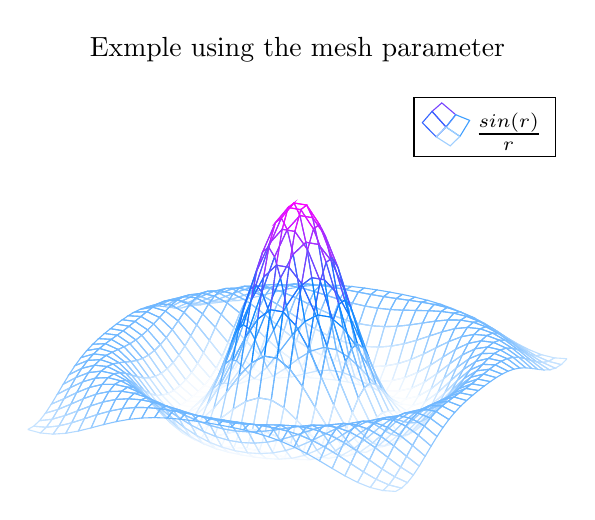
\begin{tikzpicture}
    \begin{axis}[
        title=Exmple using the mesh parameter,
        hide axis,
        colormap/cool,
    ]
    \addplot3[
        mesh,
        samples=30,
        domain=-8:8,
    ]
    {sin(deg(sqrt(x^2+y^2)))/sqrt(x^2+y^2)};
    \addlegendentry{$\frac{sin(r)}{r}$}
    \end{axis}
\end{tikzpicture}
}
    \caption{画图很慢,默认注释}
    \label{fig:my_label}
\end{figure}

\newpage
\section{符号使用规范}
参考~\cite{downes2017short,ZhangHao2017}.

\subsection{粗体}
一般而言,矩阵、向量、张量等用正粗体表示,如表~\ref{tab:math1} 所示。
\begin{table}[htbp]
    \centering
    \begin{tabular}{c c l}
        \toprule
        \LaTeX & Notation & Description   \\
        \midrule 
        \verb|a| & $a$ & 标量\\ 
        \verb|\mathbf{a}| & $\mathbf{a}$ & 向量 \\
        \verb|\mathbf{A}| & $\mathbf{A}$ & 矩阵 \\
        \verb|\mathsf{A}| & $\mathbf{A}$ & 张量 \\\bottomrule
    \end{tabular}
    \caption{数学符号规范}
    \label{tab:math1}
\end{table}

在有随机变量的情况下,为了区分随机变量和非随机变量,可以用正体表示随机变量,如表~\ref{tab:math2} 所示。
注意对于一些 \verb|\mathbf| 无法加粗的字体,可以使用 \verb|\bm| 加粗。

\begin{table}[htbp]
    \centering
    \begin{tabular}{c c l}
        \toprule
        \LaTeX & Notation & Description   \\
        \midrule 
        \verb|a| & $a$ & 标量 \\ 
        \verb|\bm{a}| & $\bm{a}$ & 向量 \\
        \verb|\bm{\mathit{A}}| & $\bm{\mathit{A}}$ & 矩阵 \\
        \verb|\bm{\mathsf{A}}| & $\bm{\mathsf{A}} $ & 张量 \\
        \verb|\mathrm{a}| & $\mathrm{a}$ & 标量随机变量 \\
        \verb|\mathbf{a}| & $\mathbf{a}$ & 向量随机变量 \\
        \verb|\mathbf{A}| & $\mathbf{A}$ & 矩阵随机变量 \\\bottomrule
    \end{tabular}
    \caption{数学符号规范(有随机变量)}
    \label{tab:math2}
\end{table}
 

\subsection{引号}
很多人平时在Word中写论文时,直接用中文输入法中的引号,例如“机器学习”,这样乍一看没什么问题,但仔细一看会发现有点别扭,因为这实际上是不规范的写法。

在 \LaTeX 中,左引号用 \verb|`|(在键盘左上角那个),右引号用 \verb|'|(键盘右边中部,平时输单双引号的键),双引号则是用两个引号,对比如下:
\begin{lstlisting}[style=latex]
    `机器', ``学习''\\
    ‘机器’, “学习”\\
\end{lstlisting}
\begin{center}
    `机器', ``学习''\\
    ‘机器’, “学习”\\
\end{center}

\subsection{算子符号}
推荐使用 \verb|\DeclareMathOperator| 定义算子,也可以临时用 \verb|\operatorname|,例如
\begin{lstlisting}[style=latex]
% 放在导言区
\DeclareMathOperator{\rank}{rank}
% 正文中
\rank(A),\qquad \operatorname{diag}(A)
\end{lstlisting}
\begin{equation*}
    \rank(A),\qquad \operatorname{diag}(A)
\end{equation*}

\subsection{函数符号}
函数的使用与算子类似,如果是一般的函数,可以用 \verb|\text|,例如
\begin{equation*}
    G^t = \text{MLP}_{t}([Q_{A}, P_{A}, Q_{X}]),\ t={1,\dots,T_o}
\end{equation*}
但如果是代码中的函数,则推荐用 \verb|\texttt|,例如
\begin{equation*}
    Q_{g} = \texttt{DeformAttn}(Q, \hat{\mathbf{x}}_{T}^{l-1}, B)
\end{equation*}

\subsection{优化问题}
\begin{lstlisting}[style=latex]
x^\star = \mathop{\arg\min}_x (x-1)^2

\begin{aligned}
    \min_{x\in \mathbb{R}^n} \quad & \quad f(x)  \\
    \mathrm{s.t.} \quad & \quad g_i(x) \le 0, \quad i = 1, 2, \ldots, m \,, \\
    & \quad h_j(x) = 0, \quad j = 1, 2, \ldots, n \,. 
\end{aligned}
\end{lstlisting}

\begin{equation*}
    x^\star = \mathop{\arg\min}_x (x-1)^2
\end{equation*}

\begin{equation*}
\begin{aligned}
\min_{x\in \mathbb{R}^n} \quad & \quad f(x)  \\
\mathrm{s.t.} \quad & \quad g_i(x) \le 0, \quad i = 1, 2, \ldots, m \,, \\
& \quad h_j(x) = 0, \quad j = 1, 2, \ldots, n \,. 
\end{aligned}
\end{equation*}




\newpage
\section{插入代码}
% 导入外部Python文件
\lstinputlisting[style=python]{code/detr.py}

% 或者直接在文档中插入代码块
\begin{lstlisting}[style=python]
# 这里是Python代码
def my_function():
    return "Hello, World!"

print(my_function())
\end{lstlisting}



\newpage
{\small
\bibliography{ref}
}

\newpage
\appendix
\section{SO(3)流形上的投影梯度}
\label{sec:SO3}
在Rotation Matrix Term中,我们要证明
\begin{equation*}
    \frac{\partial \left\| \mathbf{A}-\operatorname{proj}_{\mathcal{R}}(\mathbf{A}) \right\|_F^2}{\partial \mathbf{A}}=2\left( \mathbf{A}-\operatorname{proj}_{\mathcal{R}}(\mathbf{A}) \right)
\end{equation*}



\subsection{SVD求导}
参考SVD求导和Nuclear Norm求导的技术,我们有
\begin{equation*}
\begin{aligned}
\frac{\partial \left\| \mathbf{A}-\operatorname{proj}_{\mathcal{R}}(\mathbf{A}) \right\|_F^2}{\partial \mathbf{A}}&=\frac{\partial \left\| \mathbf{U}\bm{\Sigma}\mathbf{V}^{\top}-\mathbf{U}\mathbf{V}^{\top} \right\|_F^2}{\partial \mathbf{A}}\\
&= \frac{\partial \left\| \bm{\Sigma}-\mathbf{I} \right\|_F^2}{\partial \mathbf{A}}\\
&= \frac{\partial \operatorname{Tr}\left[ \bm{\Sigma}^2-2\bm{\Sigma}+\mathbf{I} \right] }{\partial \mathbf{A}}
\end{aligned}
\end{equation*}

由于$\mathbf{U}^{\top}\mathbf{U}=\mathbf{I},\mathbf{V}^{\top}\mathbf{V}=\mathbf{I}$,可得
\begin{equation*}
    \mathbf{U}^{\top}\mathrm{d} \mathbf{U}=\mathbf{0},\qquad \mathbf{V}^{\top}\mathrm{d} \mathbf{V}=\mathbf{0}
\end{equation*}
于是有
\begin{equation*}
\begin{aligned}
\mathrm{d}\mathbf{A}&= (\mathrm{d}\mathbf{U})\bm{\Sigma}\mathbf{V}^{\top}
+\mathbf{U}(\mathrm{d}\bm{\Sigma})\mathbf{V}^{\top}
+\mathbf{U}\bm{\Sigma}(\mathrm{d}\mathbf{V})^{\top}\\
\mathrm{d}\bm{\Sigma}&= \mathbf{U}^{\top}(\mathrm{d}\mathbf{A})\mathbf{V}
-\mathbf{U}^{\top}(\mathrm{d}\mathbf{U})\bm{\Sigma}
-\mathbf{U}^{\top}(\mathrm{d}\mathbf{V})^{\top}\mathbf{V}\\
&= \mathbf{U}^{\top}(\mathrm{d}\mathbf{A})\mathbf{V}
\end{aligned}
\end{equation*}

最终,我们有
\begin{equation*}
\begin{aligned}
\frac{\partial \operatorname{Tr}\left[ \bm{\Sigma}^2-2\bm{\Sigma}+\mathbf{I} \right] }{\partial \mathbf{A}}&= \frac{\operatorname{Tr}\left[ 2(\bm{\Sigma}-\mathbf{I})\partial \bm{\Sigma} \right] }{\partial \mathbf{A}}\\
&= \frac{\operatorname{Tr}\left[ 2(\bm{\Sigma}-\mathbf{I})\mathbf{U}^{\top}(\partial\mathbf{A})\mathbf{V} \right] }{\partial \mathbf{A}}\\
&= \frac{\operatorname{Tr}\left[ 2\mathbf{V}(\bm{\Sigma}-\mathbf{I})\mathbf{U}^{\top}(\partial\mathbf{A}) \right] }{\partial \mathbf{A}}\\
&= 2\mathbf{U}(\bm{\Sigma}-\mathbf{I})\mathbf{V}^{\top}\\
&= 2(\mathbf{A}-\mathbf{U}\mathbf{V}^{\top})\\
&= 2(\mathbf{A}-\operatorname{proj}_{\mathcal{R}}(\mathbf{A}))
\end{aligned}
\end{equation*}



\end{document}
